% Options for packages loaded elsewhere
\PassOptionsToPackage{unicode}{hyperref}
\PassOptionsToPackage{hyphens}{url}
%
\documentclass[
]{book}
\usepackage{amsmath,amssymb}
\usepackage{iftex}
\ifPDFTeX
  \usepackage[T1]{fontenc}
  \usepackage[utf8]{inputenc}
  \usepackage{textcomp} % provide euro and other symbols
\else % if luatex or xetex
  \usepackage{unicode-math} % this also loads fontspec
  \defaultfontfeatures{Scale=MatchLowercase}
  \defaultfontfeatures[\rmfamily]{Ligatures=TeX,Scale=1}
\fi
\usepackage{lmodern}
\ifPDFTeX\else
  % xetex/luatex font selection
\fi
% Use upquote if available, for straight quotes in verbatim environments
\IfFileExists{upquote.sty}{\usepackage{upquote}}{}
\IfFileExists{microtype.sty}{% use microtype if available
  \usepackage[]{microtype}
  \UseMicrotypeSet[protrusion]{basicmath} % disable protrusion for tt fonts
}{}
\makeatletter
\@ifundefined{KOMAClassName}{% if non-KOMA class
  \IfFileExists{parskip.sty}{%
    \usepackage{parskip}
  }{% else
    \setlength{\parindent}{0pt}
    \setlength{\parskip}{6pt plus 2pt minus 1pt}}
}{% if KOMA class
  \KOMAoptions{parskip=half}}
\makeatother
\usepackage{xcolor}
\usepackage{color}
\usepackage{fancyvrb}
\newcommand{\VerbBar}{|}
\newcommand{\VERB}{\Verb[commandchars=\\\{\}]}
\DefineVerbatimEnvironment{Highlighting}{Verbatim}{commandchars=\\\{\}}
% Add ',fontsize=\small' for more characters per line
\usepackage{framed}
\definecolor{shadecolor}{RGB}{248,248,248}
\newenvironment{Shaded}{\begin{snugshade}}{\end{snugshade}}
\newcommand{\AlertTok}[1]{\textcolor[rgb]{0.94,0.16,0.16}{#1}}
\newcommand{\AnnotationTok}[1]{\textcolor[rgb]{0.56,0.35,0.01}{\textbf{\textit{#1}}}}
\newcommand{\AttributeTok}[1]{\textcolor[rgb]{0.13,0.29,0.53}{#1}}
\newcommand{\BaseNTok}[1]{\textcolor[rgb]{0.00,0.00,0.81}{#1}}
\newcommand{\BuiltInTok}[1]{#1}
\newcommand{\CharTok}[1]{\textcolor[rgb]{0.31,0.60,0.02}{#1}}
\newcommand{\CommentTok}[1]{\textcolor[rgb]{0.56,0.35,0.01}{\textit{#1}}}
\newcommand{\CommentVarTok}[1]{\textcolor[rgb]{0.56,0.35,0.01}{\textbf{\textit{#1}}}}
\newcommand{\ConstantTok}[1]{\textcolor[rgb]{0.56,0.35,0.01}{#1}}
\newcommand{\ControlFlowTok}[1]{\textcolor[rgb]{0.13,0.29,0.53}{\textbf{#1}}}
\newcommand{\DataTypeTok}[1]{\textcolor[rgb]{0.13,0.29,0.53}{#1}}
\newcommand{\DecValTok}[1]{\textcolor[rgb]{0.00,0.00,0.81}{#1}}
\newcommand{\DocumentationTok}[1]{\textcolor[rgb]{0.56,0.35,0.01}{\textbf{\textit{#1}}}}
\newcommand{\ErrorTok}[1]{\textcolor[rgb]{0.64,0.00,0.00}{\textbf{#1}}}
\newcommand{\ExtensionTok}[1]{#1}
\newcommand{\FloatTok}[1]{\textcolor[rgb]{0.00,0.00,0.81}{#1}}
\newcommand{\FunctionTok}[1]{\textcolor[rgb]{0.13,0.29,0.53}{\textbf{#1}}}
\newcommand{\ImportTok}[1]{#1}
\newcommand{\InformationTok}[1]{\textcolor[rgb]{0.56,0.35,0.01}{\textbf{\textit{#1}}}}
\newcommand{\KeywordTok}[1]{\textcolor[rgb]{0.13,0.29,0.53}{\textbf{#1}}}
\newcommand{\NormalTok}[1]{#1}
\newcommand{\OperatorTok}[1]{\textcolor[rgb]{0.81,0.36,0.00}{\textbf{#1}}}
\newcommand{\OtherTok}[1]{\textcolor[rgb]{0.56,0.35,0.01}{#1}}
\newcommand{\PreprocessorTok}[1]{\textcolor[rgb]{0.56,0.35,0.01}{\textit{#1}}}
\newcommand{\RegionMarkerTok}[1]{#1}
\newcommand{\SpecialCharTok}[1]{\textcolor[rgb]{0.81,0.36,0.00}{\textbf{#1}}}
\newcommand{\SpecialStringTok}[1]{\textcolor[rgb]{0.31,0.60,0.02}{#1}}
\newcommand{\StringTok}[1]{\textcolor[rgb]{0.31,0.60,0.02}{#1}}
\newcommand{\VariableTok}[1]{\textcolor[rgb]{0.00,0.00,0.00}{#1}}
\newcommand{\VerbatimStringTok}[1]{\textcolor[rgb]{0.31,0.60,0.02}{#1}}
\newcommand{\WarningTok}[1]{\textcolor[rgb]{0.56,0.35,0.01}{\textbf{\textit{#1}}}}
\usepackage{longtable,booktabs,array}
\usepackage{calc} % for calculating minipage widths
% Correct order of tables after \paragraph or \subparagraph
\usepackage{etoolbox}
\makeatletter
\patchcmd\longtable{\par}{\if@noskipsec\mbox{}\fi\par}{}{}
\makeatother
% Allow footnotes in longtable head/foot
\IfFileExists{footnotehyper.sty}{\usepackage{footnotehyper}}{\usepackage{footnote}}
\makesavenoteenv{longtable}
\usepackage{graphicx}
\makeatletter
\def\maxwidth{\ifdim\Gin@nat@width>\linewidth\linewidth\else\Gin@nat@width\fi}
\def\maxheight{\ifdim\Gin@nat@height>\textheight\textheight\else\Gin@nat@height\fi}
\makeatother
% Scale images if necessary, so that they will not overflow the page
% margins by default, and it is still possible to overwrite the defaults
% using explicit options in \includegraphics[width, height, ...]{}
\setkeys{Gin}{width=\maxwidth,height=\maxheight,keepaspectratio}
% Set default figure placement to htbp
\makeatletter
\def\fps@figure{htbp}
\makeatother
\setlength{\emergencystretch}{3em} % prevent overfull lines
\providecommand{\tightlist}{%
  \setlength{\itemsep}{0pt}\setlength{\parskip}{0pt}}
\setcounter{secnumdepth}{5}
\usepackage{booktabs}
\ifLuaTeX
  \usepackage{selnolig}  % disable illegal ligatures
\fi
\usepackage[]{natbib}
\bibliographystyle{plainnat}
\usepackage{bookmark}
\IfFileExists{xurl.sty}{\usepackage{xurl}}{} % add URL line breaks if available
\urlstyle{same}
\hypersetup{
  pdftitle={Machine Learning in Genomics: Containerised tutorials demonstrating best practises, pitfalls, and reproducibility},
  pdfauthor={ Sach Nehal},
  hidelinks,
  pdfcreator={LaTeX via pandoc}}

\title{Machine Learning in Genomics: Containerised tutorials demonstrating best practises, pitfalls, and reproducibility}
\author{Sach Nehal}
\date{2024-09-02}

\begin{document}
\maketitle

{
\setcounter{tocdepth}{1}
\tableofcontents
}
\chapter*{About}\label{about}
\addcontentsline{toc}{chapter}{About}

Applied machine learning utilising vast amounts of data has aided in pattern identification, predictive analytics, and solving complex problems across a multitude of fields. Solving these complex problems within these fields, researchers would find differing answers to the following questions; \textbf{what machine learning techniques can we apply to the problem, how do we apply the techniques in the context of this field, and why do we need to apply them in this way?} In any case, applied machine learning requires an interdisciplinary understanding of computing techniques and the field in question.

The aim of this project is to provide you with \textbf{a set of reproducible, containerized tutorials that include all necessary data, code, and descriptions to replicate key results, along with demonstrations of common pitfalls, in the field of genomics}. It is designed for users with knowledge of machine learning but little or no background in biology as a process to learn about applying machine learning techniques in genomics.

\part{Introduction}\label{part-introduction}

\chapter{Epigenetic Data}\label{epigenetic-data}

\section{What is epigenetic data?}\label{what-is-epigenetic-data}

As you may already know, typically all of the cells in your body contain the same DNA. How, then, do we have different cell types in our body? Your DNA contains a script that is able to produce the proteins required for each specific cell in your body. Which proteins, and subsequently which cells are made, depends on gene expression and regulation, i.e.~``the way each cell deploys its genome.''\footnote{\citet{ralston2008}}

\textbf{\emph{Epigenetic data}} arises from ``the study of heritable and stable changes in gene expression that occur through alterations in the chromosome rather than in the DNA sequence.''\footnote{\citet{nora2023}}

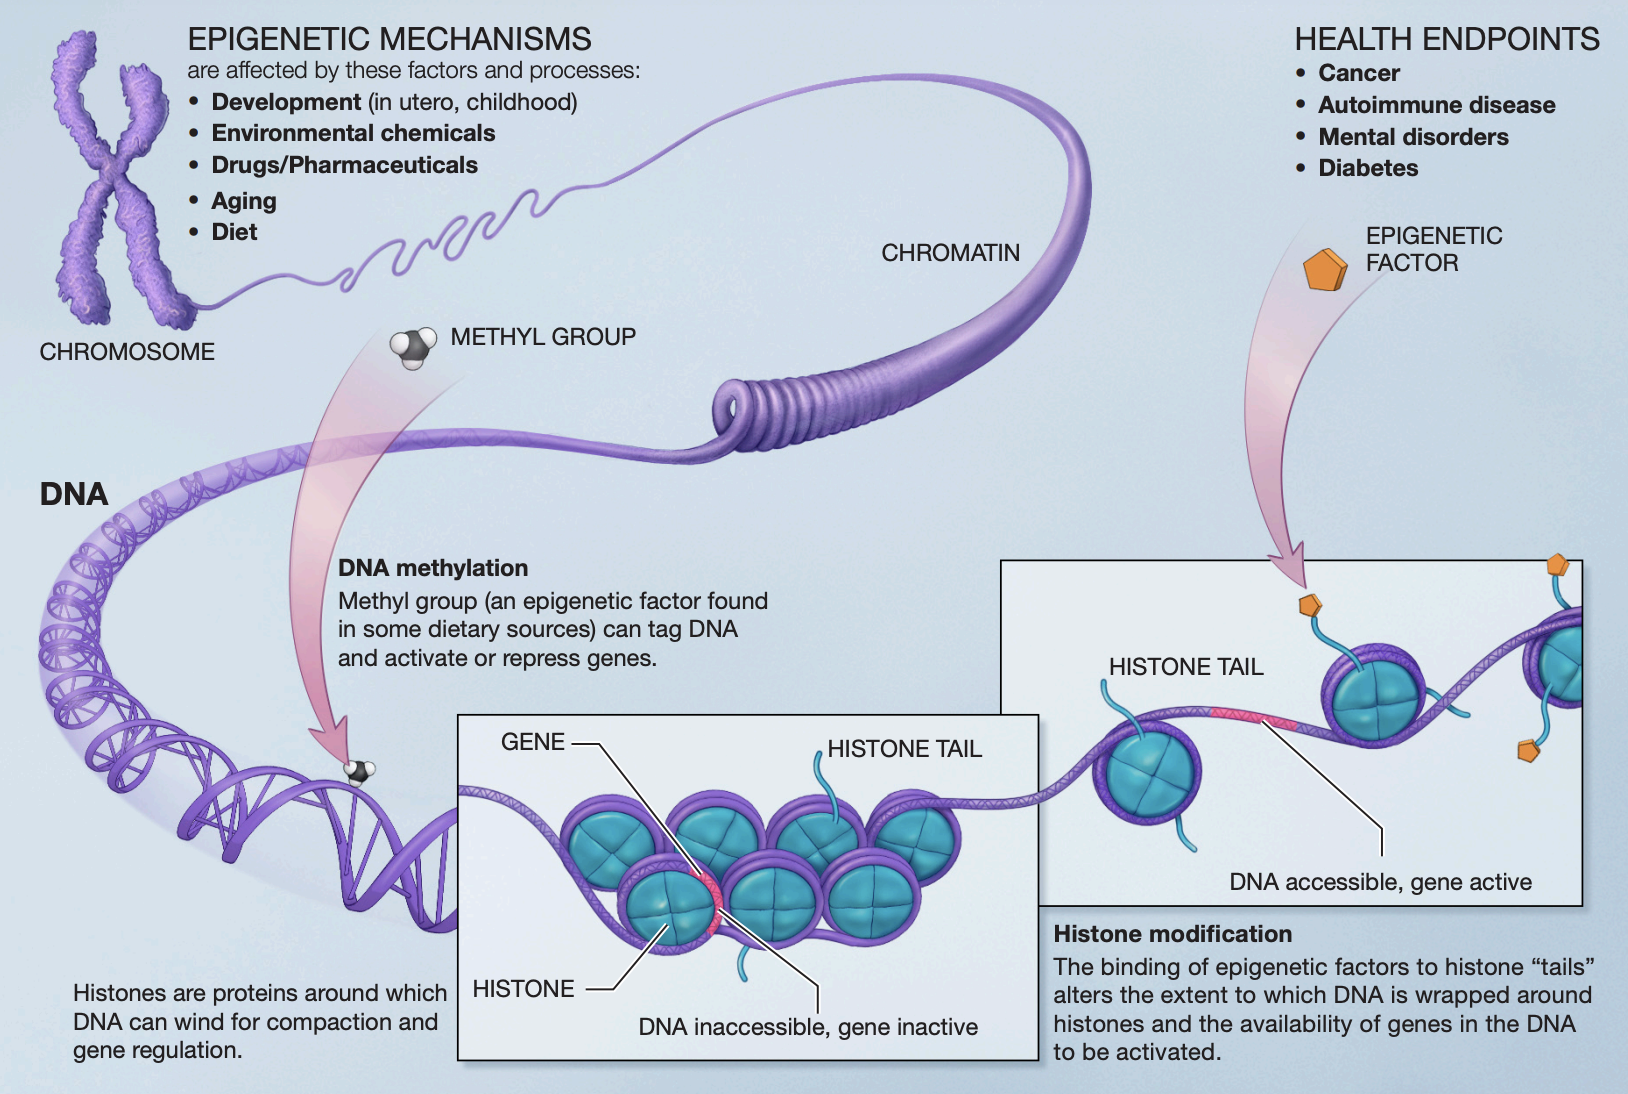
\includegraphics{images/Epigenetic_Mechanisms.png}

\href{https://commonfund.nih.gov/sites/default/files/epigeneticmechanisms.pdf}{commonfund.nih.gov}

The image above shows quite simply the basics of genetic structures. Several more complex processes are involved during cell replication such as DNA transcription and translation in order to make proteins. A key takeaway in coming closer to understanding gene expression is that \textbf{Chromatin} is a complex structure made up of DNA wound around histone proteins, with some segments of DNA being accessible/inaccessible to further processes. \textbf{Euchromatin} refers to the accessible state, while \textbf{Heterochromatin} refers to a chromatin state in which DNA cannot be transcribed (inaccessible).\footnote{\citet{shahid2023}} There are many different epigenetic modifications that affect chromatin accessibility.

Some common epigenetic modifications include:

\begin{enumerate}
\def\labelenumi{\arabic{enumi}.}
\tightlist
\item
  \textbf{DNA Methylation}: Addition of methyl groups to DNA, affecting gene expression regulation\footnote{\citet{nora2023}}.
\item
  \textbf{Histone Modifications}: Chemical changes to histone proteins that DNA wraps around, including acetylation, methylation, or phosphorylation. These changes influence chromatin structure and gene accessibility.\footnote{\citet{Kouzarides2007}}
\item
  \textbf{Chromatin Accessibility}: Regions of open chromatin that are accessible to transcription factors (special types of proteins that bind to DNA sequences and regulate gene expression) further dictate which regions of DNA can be expressed\footnote{\citet{melanie2021}}.
\end{enumerate}

In studying gene expression and epigenetic modifications, we aim to more closely understand biological mechanisms that regulate development, disease, and how cells respond to epigenetic factors.

\subsection{What Does DNA Look Like?}\label{what-does-dna-look-like}

As illustrated in the image above, DNA is structured as a double helix, with two complementary strands intertwined to form the characteristic helical shape. DNA consists of an extremely long sequence composed of four types of nucleotides: Adenine (A), Cytosine (C), Thymine (T), and Guanine (G).

According to the National Cancer Institute (USA), nucleotides within the DNA double helix form complementary pairs---Adenine pairs with Thymine, and Guanine pairs with Cytosine\footnote{\citet{ncidefinitions}}. These pairs are commonly referred to as base pairs (bps). For example, if one strand of the double helix has the sequence ``ATCGG'', the complementary strand will have the sequence ``TAGCC''.

Genes are sequences of DNA located at specific positions on chromosomes and can vary in length. Each gene encodes information necessary for producing proteins or RNA molecules, which are essential for the structure, function, and regulation of an organism\footnote{\citet{ncidefinitions}}. The complete set of genetic material in an organism is known as its genome.

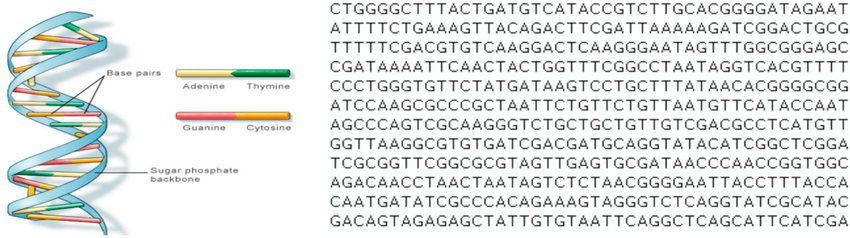
\includegraphics{images/dna_sequence.png}

Image highlighting part of a \href{https://www.researchgate.net/profile/Pratik-Kanani/publication/341901570/figure/fig1/AS:898621708984321@1591259519483/A-human-DNA-and-Part-of-DNA-sequence-28-29.jpg}{dna sequence and base pairs}.\footnote{\citet{kanani2020}}

\subsection{Common Epigenetic Sequencing Techniques:}\label{common-epigenetic-sequencing-techniques}

\begin{enumerate}
\def\labelenumi{\arabic{enumi}.}
\item
  \textbf{\emph{ATAC-Seq}} (Assay for Transposase-Accessible Chromatin with Sequencing):
  o\texttt{Measures\ chromatin\ accessibility\ to\ identify\ open\ regions\ of\ the\ genome\ where\ transcription\ factors\ can\ bind.}
  o\texttt{Output:\ Peaks\ indicating\ accessible\ chromatin\ regions.}
\item
  \textbf{\emph{ChIP-Seq}} (Chromatin Immunoprecipitation Sequencing):
  o\texttt{Used\ to\ identify\ DNA\ regions\ bound\ by\ specific\ proteins\ (e.g.,\ transcription\ factors,\ histones\ with\ specific\ modifications).}
  o\texttt{Output:\ Peaks\ indicating\ binding\ sites\ or\ modification\ locations.}
\end{enumerate}

\section{What does epigenetic data look like?}\label{what-does-epigenetic-data-look-like}

Epigenetic data can be represented in various forms, depending on the type of modification being studied and the methods used to gather the data. \textbf{ATAC-Seq} and \textbf{ChIP-Seq} are the common methods I will focus on, but there are others that may produce different forms of data, such as WGS (whole-genome sequencing) which produces nucleotide sequencing data, or Bisulfite conversion of DNA producing data on methylation levels across the genome.

\subsection{Representing epigenetic data}\label{representing-epigenetic-data}

Epigenetic data originates from sequencing methods such as ATAC-Seq or ChIP-Seq experiments. The initial experiments produce raw sequencing reads (fragments), which are then aligned to a reference genome. By aligning these sequences, we can aggregate the reads into regions where they `pile up' to form peaks, indicating areas of significant biological activity or modification. This can be done per base across the genome, or per gene. Additionally, we could also examine mismatches where a read's base differs from the genome's base, and use them to identify SNPs (\href{https://www.cancer.gov/publications/dictionaries/genetics-dictionary/def/single-nucleotide-polymorphism}{single nucleotide polymorphisms})\footnote{\citet{ncidefinitions}}. This mismatch information can be recorded in a table showing the position, type of mismatch, and the number of reads supporting each mismatch.\footnote{\citet{akalin2020}}

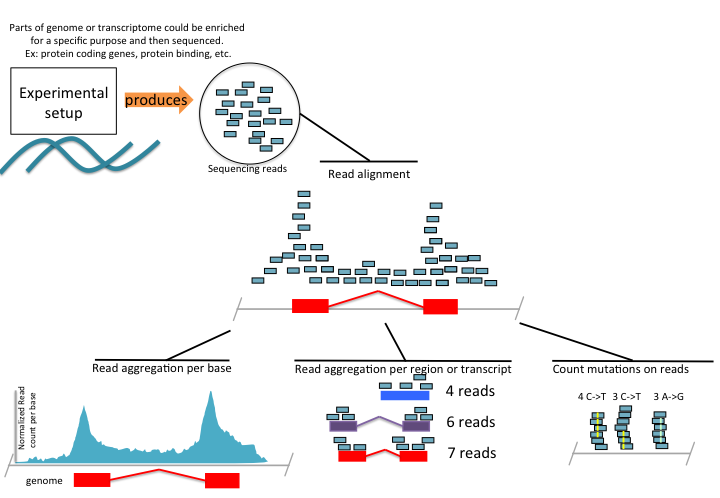
\includegraphics{images/sequencing_pipeline.png}

Image showing the \href{https://compgenomr.github.io/book/images/HTseq.png}{sequencing pipeline} from high-throughput sequencing methods\footnote{\citet{akalin2020}}.

1. \textbf{\emph{Raw Sequence Reads:}}
o\texttt{These\ are\ the\ basic\ output\ of\ sequencing\ experiments,\ such\ as\ those\ from\ ChIP-Seq\ or\ ATAC-Seq.}
o\texttt{Reads\ are\ processed\ and\ aligned\ to\ a\ reference\ genome\ before\ undergoing\ peak\ calling.}

Lets look at what a few lines of raw sequence read data consists of:
The data is taken from Encode Experiment \href{https://www.encodeproject.org/experiments/ENCSR817LUF/}{ENCSR817LUF} (chIP-Seq). The accession ID of the raw sequence read data is \href{https://www.encodeproject.org/files/ENCFF397NRK/}{ENCFF397NRK}. Genomic data comes in many file formats. This specific raw sequence read data is a compressed FASTQ file.

Note: The script I used involved streaming the data directly from a URL using the requests library. While files containing genomic data are generally quite large, for computational efficiency it is recommended that data be downloaded locally.

\begin{verbatim}
## ID: B091JABXX110402:1:2204:12975:184709
## Sequence: GTTAGGGTTAGGGTTAGGGTTAGGGTTAGGGTTAGG
## Quality Scores: [31, 30, 30, 32, 36, 37, 36, 32, 33, 32, 35, 36, 37, 33, 33, 34, 37, 37, 36, 33, 34, 30, 37, 37, 37, 33, 34, 33, 38, 33, 33, 32, 33, 35, 37, 36]
## 
## ID: B091JABXX110402:1:2205:18641:8399
## Sequence: GGTTAGGGTTAGGGTTAGGGTTAGGGTTAGGGTTAG
## Quality Scores: [22, 27, 31, 30, 30, 33, 31, 32, 31, 31, 24, 36, 37, 36, 33, 34, 33, 37, 37, 32, 32, 34, 22, 37, 36, 30, 23, 35, 27, 29, 28, 28, 23, 31, 26, 35]
## 
## ID: B091JABXX110402:1:1207:12202:100922
## Sequence: AGGGTTAGGGTTAGGGTTAGGGTTAGGGTTAGGGTT
## Quality Scores: [33, 33, 36, 37, 31, 34, 34, 36, 37, 36, 29, 33, 35, 36, 39, 37, 32, 33, 35, 37, 34, 37, 33, 34, 36, 38, 39, 25, 32, 35, 36, 38, 37, 38, 32, 32]
\end{verbatim}

As you can see, each data entry is a DNA sequence (read). While I'm only showing the first three entries, for each experiment there are millions of sequencing reads. The quality scores indicate the confidence of each base call in the sequence. Higher scores suggest higher confidence. The scores are in Phred format, where a score of 20 corresponds to a 99\% base call accuracy, 30 corresponds to 99.9\%, 40 corresponds to 99.99\%, and so on.\footnote{\citet{green}}
2. \textbf{\emph{Peak Calling:}}
o\texttt{A\ method\ used\ to\ identify\ regions\ in\ the\ genome\ where\ there\ is\ significant\ enrichment\ of\ sequencing\ reads.\ This\ indicates\ the\ presence\ of\ DNA-protein\ interactions\ (e.g.,\ transcription\ factor\ binding\ sites\ or\ accessible\ chromatin\ regions).}
o\texttt{Peaks\ represent\ areas\ where\ epigenetic\ marks\ or\ chromatin\ accessibility\ are\ concentrated.}

A common peak calling algorithm is \href{https://hbctraining.github.io/Intro-to-ChIPseq/lessons/05_peak_calling_macs.html}{MACS2}. Essentially, aligned sequencing reads are aggregated into regions where they `pile up' to form peaks as a read count per base. The outputs typically include signal p-values or fold change over control values, representing the expectation of a peak. Signal p-values are negative log transformed resulting in -log10 signal p-values. While MACS2 is traditionally used in ChIP-seq experiments, it is also applied to ATAC-seq to identify significant peaks and assess their enrichment.\footnote{\citet{mistry2022}} In ChIP-seq, broad peaks often represent histone modifications covering entire gene bodies, while narrow peaks are indicative of transcription factor binding sites. In ATAC-seq, the peaks primarily reflect regions of open chromatin.\footnote{\citet{wilbanks2010}} Peak calling reduces background noise and utilises signal smoothing techniques to more accurately detect peaks. When using -log10 p-value and fold change data, base pair averaging is commonly used.

Imagine you have a set of read coverage data from a sequencing experiment. At each base pair position along a chromosome, you have a read count representing how many times that base pair was sequenced. However, due to technical noise, these counts might fluctuate wildly from one base to the next. By applying base pair averaging over a window (e.g.~32bp), you might see that while individual counts vary, there is a broader region where the average read coverage is consistently high, indicating a potential region of interest. The intended effect of base pair averaging is further reducing noise, and signal smoothing.
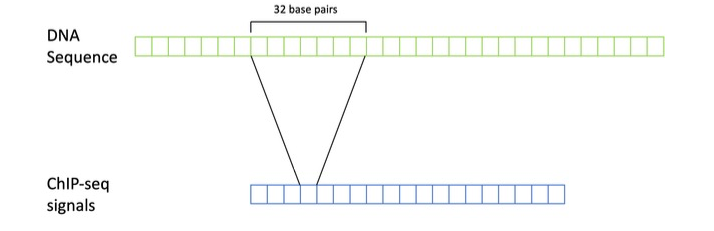
\includegraphics{images/bp_resolution.png}

Figure showing a 32 base pair resolution following base pair averaging of CHip-seq data\footnote{\citet{patel2024}}

As you will see in the tutorials, you can re-average your data to a higher base pair average before using it in machine learning models. This can be implemented to decrease dimensionality, reduce computational intensity and tailor the model to understanding regions of a certain scale.

\textbf{\emph{Representing Peaks:}}
o \textbf{\emph{P-value or Fold-change:}}
P-value: Indicates the statistical significance of the peak, helping to distinguish true peaks from background noise.
Fold-change: Represents the difference in read density between treated and control samples, indicating the strength of the signal.

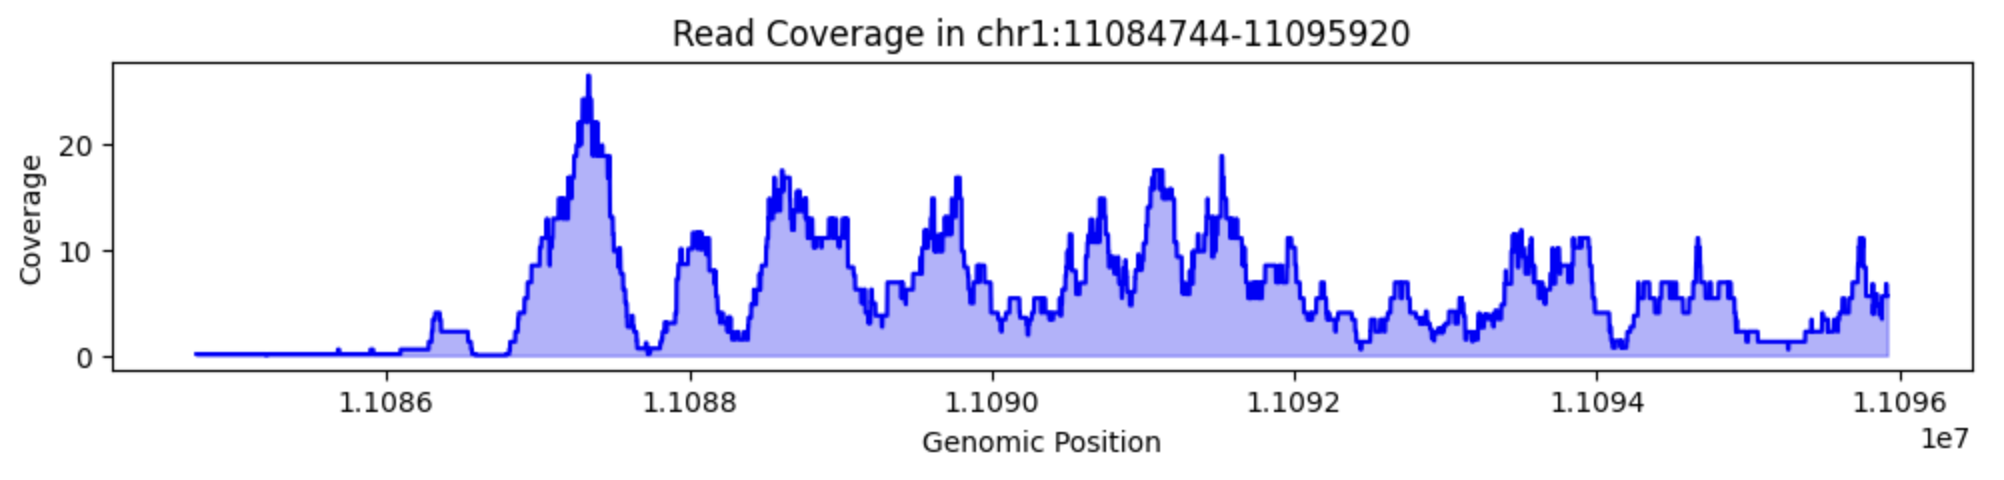
\includegraphics{images/coverage_p.png}
This image shows the signal p-value coverage over a small region (11,176bps) in chromosome one from Encode Experiment \href{https://www.encodeproject.org/experiments/ENCSR817LUF/}{ENCSR817LUF} (The same chIP-Seq experiment we saw the raw sequence reads from). For further context, experiment ENCSR817LUF targets the H3K36me3 histone modification in brain tissue. The experiment aims to map the locations where the H3K36me3 histone modification is present along the genome. Therefore the peaks represent regions of the genome where the the H3K36me3 histone modification is enriched compared to the background or control. The accession ID of the signal p-value data is \href{https://www.encodeproject.org/files/ENCFF601VTB/}{ENCFF601VTB}. Genomic data comes in many file formats. This specific signal p-value data is a bigWig file.
o \textbf{\emph{Types of Peaks:}}
Categorical Peaks: Simple yes/no indication of a peak's presence.
Continuous Peaks: More nuanced representation that includes the intensity or enrichment level of the peak, often visualized as a signal track.
Thresholded/Pseudoreplicated Peaks: Usually categorical, these peaks are of high confidence regions from multiple replicates (experiments) or pseudoreplicates (artificial data splits), to ensure reliability and reproducibility.

\textbf{\emph{Example Data Pipeline}}

\href{https://www.encodeproject.org/experiments/ENCSR817LUF/}{encodeproject.org}

This is an example data pipeline from Encode Experiment \href{https://www.encodeproject.org/experiments/ENCSR817LUF/}{ENCSR817LUF}, the same chIP-Seq experiment we saw the raw sequence reads, and signal p-value coverage from. The yellow bubbles represent downloadable data sets of different types, while the blue boxes represent step types (e.g.~peak calling). In the left column are multiple data sets of raw sequence reads, which then undergo data quality steps before being aligned (first blue box) to the reference human genome GRCh38 (denoted by ENCFF110MCL below the reads). The next steps include Peak calling (categorical peaks) and signal generation (continuous peaks) to produce the data we normally use in our machine learning models. This data pipeline process aids in normalisation, noise reduction, and dimensionality reduction of the data.

\subsection{Transformations to stop extreme p-values}\label{transformations-to-stop-extreme-p-values}

When utlising genomic data which incorporates p-values, it is important to consider and deal with extreme p-values. One way this is done is through using an Arcsinh-transformation (inverse hyperbolic sine).
\(\text{arsinh}(x) = \ln \left( x + \sqrt{x^2 + 1} \right)\)

The arcsinh-transformation as a logarithmic function helps in reducing the significance of outliers and sequencing depth while maintaining variance by compressing the range of the data. This transformation can be used in the data preprocessing stage. The graph below visualises how the transformation works. While extreme values are transformed logarithmically, the smaller values are barely transformed as the function for smaller values is more linear in nature.

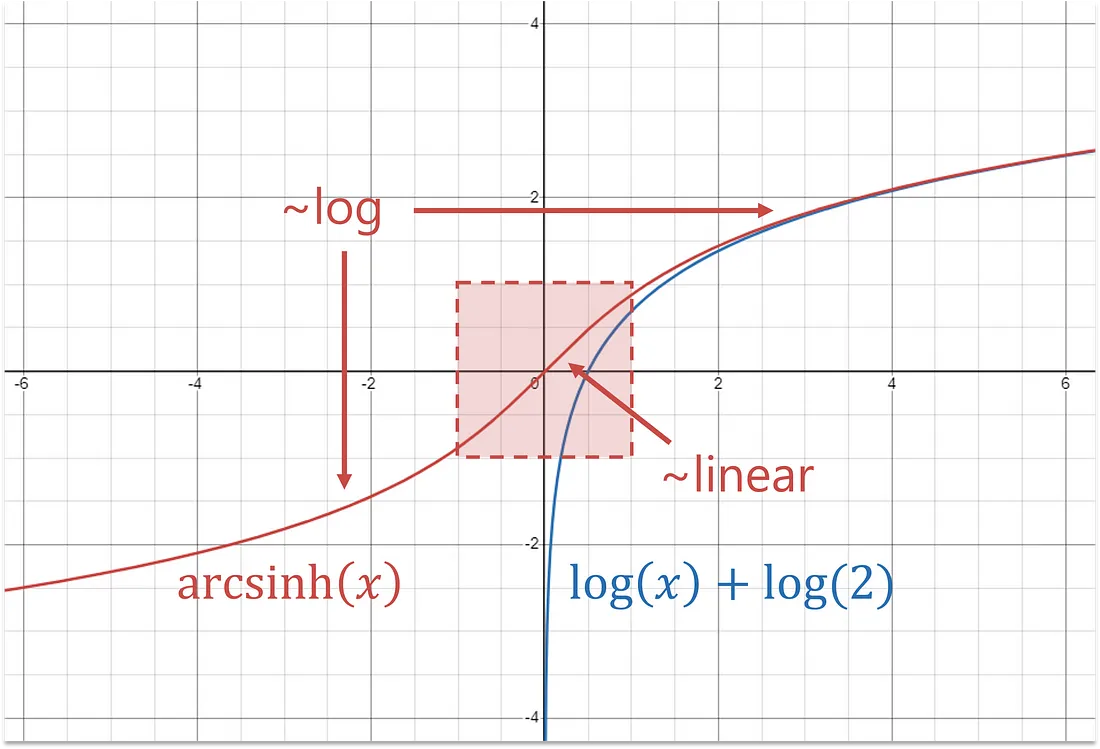
\includegraphics{images/arcsinh.png}

Plot of \href{https://miro.medium.com/v2/resize:fit:1100/format:webp/1*glJtHk1HRZpYHsk79QxgwQ.png}{Arcsinh Transformation} compared to a log function, made with Desmos available under \href{https://miro.medium.com/v2/resize:fit:1100/format:webp/1*glJtHk1HRZpYHsk79QxgwQ.png}{CC BY-SA 4.0.} Text, arrows, and box shape added to image.

\section{Sources of epigenetic data}\label{sources-of-epigenetic-data}

There are numerous public data banks which contain genomic datasets ready to be downloaded.
\href{https://projects.ensembl.org/blueprint/}{Blueprint}
Blueprint's genomic datasets are focused on gene expression in healthy and diseased cells mostly relating to haematopoietic cells (cells which develop into different types of blood cells).

\href{https://www.ncbi.nlm.nih.gov/geo/roadmap/epigenomics/}{Roadmap}
The National Institute of Health's Roadmap Epigenomics Project contains sample datasets from multiple experiements as well as reference and mapping datasets.

\href{https://www.encodeproject.org/}{Encode}
The Encode Project contains a large amount of publicly available genomic data easily filtered and downloaded. The genomic data used in this markdown book is sourced from Encode.

The largest genomic data bank is the \href{https://www.ukbiobank.ac.uk/}{UK Biobank}, however they require that you apply for access to their datasets.

\section{UCSC'S Genome Browser}\label{ucscs-genome-browser}

The UCSC Genome Browser is a powerful and versatile tool that allows the visualisation and exploration of many sets of genomic data, especially bigWig files. It offers an extensive collection of genome assemblies, annotation tracks, and functional data, enabling users to examine gene structures, regulatory elements, and genetic variations. With its user-friendly interface and customisable display options, the UCSC Genome Browser facilitates detailed genomic analyses and supports a wide range of applications in genomics and bioinformatics. Whether you're investigating gene functions, exploring genetic variants, or studying comparative genomics, the UCSC Genome Browser serves as an essential resource for understanding complex genomic information. It is also possible to load and visualise genomic data from other sources such as Encode. While the visualisations are extensive, as you can explore below, the browser can be quite overwhelming for first time users.

The following is an example of what the same chIP-Seq data targeting the H3K36me3 histone modification in brain tissue looks like using UCSC's Genome Browser. The pseudoreplicated peaks represent categorically, the significant locations along the genome where the H3K36me3 histone modification is present.

\href{https://genome.ucsc.edu/cgi-bin/hgTracks?db=hg38&lastVirtModeType=default&lastVirtModeExtraState=&virtModeType=default&virtMode=0&nonVirtPosition=&position=chr1\%3A11084744\%2D11095920&hgsid=2307713234_Kap236Tjt6ZGnnNrXMkIhq2Ajn27}{UCSC Genome Browser}

The following is an example of ATAC-Seq data from an experiment on T-helper 17 cells (a type of immune system cell). Recall that the ATAC-Seq method aims to find chromatin regions that are accessible for transcription factor binding. The p-value and fold change graphs show continuous peaks, while the IDR thresholded peaks and pseudoreplicated peaks represent the significant locations of accessible chromatin along the genome.

\href{https://genome.ucsc.edu/cgi-bin/hgTracks?db=hg38&lastVirtModeType=default&lastVirtModeExtraState=&virtModeType=default&virtMode=0&nonVirtPosition=&position=chr1\%3A88379533\%2D113275174&hgsid=2307721306_mcnECXS4Hy0fNQ4yz3ZQTL7nimkW}{UCSC Genome Browser}

\chapter{Pre-processing of bigWig files}\label{pre-processing-of-bigwig-files}

BigWig files containing signal p-value or fold change data can be quite tricky to deal with. However, libraries such as pyBigWig enable easier access of data. In order to understand how to handle the data pre-processing stage, I have created a jupyter notebook tutorial on Google Colab. The tutorial begins using UCSC's programs to quickly understand the genomic data within BigWigs, before using the pyBigWig library to simply extract BigWig data.

The final part of the tutorial uses the pyBigWig library to load, filter, and split BigWig data into training, validation, and test sets. The data consists of signal p-values from ChIP-seq experiments, processed using the MACS2 tool. We will re-average these signals to a resolution of 32 base pairs. Additionally, we will implement threshold-based filtering and consistent data splits to understand how to ready data for a model.

Tutorial 1: Loading and Pre-Processsing Data from bigWigs (interactive)

Tutorial 1: Loading and Pre-Processsing Data from bigWigs (nbviewer)

\section{Data loaders and simplifying pre-processing}\label{data-loaders-and-simplifying-pre-processing}

Data loaders are scripts/functions to load batches of data into your model. They are crucial in machine learning because they simplify how data is fed into models, making the whole process smoother and more efficient. This becomes especially important with the large datasets used in genomic studies, where managing and processing data manually would be cumbersome. By automating these tasks, data loaders help ensure that data is processed efficiently, allowing for faster and more effective model training. While there are existing github repositories with data loaders, such as \href{https://kipoi.org/kipoiseq/dataloaders/}{``Kipoi Dataloader''}, and \href{https://github.com/pfizer-opensource/bigwig-loader/blob/main/README.md}{``Dataloader for BigWig files''}.\footnote{\citet{retel_fast_2024}}, depending on the data used and model you build, they won't cover all of the use cases. When building one yourself, the PyTorch library has its own \href{https://pytorch.org/tutorials/beginner/basics/data_tutorial.html}{dataset and dataloader} modules, which include creating custom datasets.

\section{Dealing with missing data (oversampling, undersampling, weighting)}\label{dealing-with-missing-data-oversampling-undersampling-weighting}

In genomics, class imbalance is a frequent challenge, often necessitating the use of statistical methods to validate the few positive instances amid vast amounts of data. This is particularly evident in tasks such as alignment queries, GWAS projects, and motif scanning, where conservative significance thresholds are essential to control false positives due to the low frequency of true positives across the genome. Researchers tend to address these imbalances by either oversampling the minority class, undersampling the majority class or by employing weighting.\footnote{\citet{whalen2022}}

In Tutorial 1, we utilised thresholding to filter our data to focus on regions with significant coverage. While there were around 300,000 bins across the three chromosomes we looked at, after thresholding our data consisted of roughly 10\% or 30,000 bins. Our data does not contain any coverage values below the threshold. In the pitfalls section, we will explore how a model performs with and without regions of zero signal.

Methods for dealing with class imbalances:

\begin{itemize}
\item
  \href{https://imbalanced-learn.org/stable/user_guide.html\#user-guide}{Scikit-learn's `imbalance-learn' package} (Oversampling, Undersampling and Weighting)
  ``Imbalanced-learn (imported as imblearn) is an open source, MIT-licensed library relying on scikit-learn (imported as sklearn) and provides tools when dealing with classification with imbalanced classes.''
\item
  \href{https://machinelearningmastery.com/smote-oversampling-for-imbalanced-classification/}{SMOTE} (Oversampling)
  ``a random example from the minority class is first chosen. Then k of the nearest neighbors for that example are found (typically k=5). A randomly selected neighbor is chosen and a synthetic example is created at a randomly selected point between the two examples in feature space.''
\item
  \href{https://imbalanced-learn.org/stable/references/generated/imblearn.over_sampling.ADASYN.html}{ADASYN} (Oversampling)
  ``similar to SMOTE but it generates different number of samples depending on an estimate of the local distribution of the class to be oversampled.''
\end{itemize}

\part{Training models with DNA input}\label{part-training-models-with-dna-input}

\chapter{Loss functions, and peak metrics}\label{loss-functions-and-peak-metrics}

When selecting the optimal loss function for your machine learning model in genomics, the decision should be informed by the nature of the problem and the specific type of data you're working with. The principles for choosing loss functions in genomics are similar to those in other machine learning contexts. For regression based tasks, while Mean Squared Error (mse) loss functions have been used, models utilising data and making predictions associated with reads or counts use a Poisson loss function. Another two common loss functions include Binary Cross-Entropy loss and Categorical Cross-Entropy loss, when dealing with classification type predictions.\footnote{\citet{patterson2017}}

\textbf{Mean Squared Error (MSE):}
• Use Case: Regression problems where the goal is to predict continuous values, such as gene expression or coverage levels.
Example: \href{https://genomebiology.biomedcentral.com/articles/10.1186/s13059-019-1837-6}{DeepImpute}, a deep neural network-based imputation algorithm that allows for accurate imputation of single-cell RNA-seq data. The model is used to estimate missing or low-quality gene expression values in single-cell RNA sequencing datasets. It uses a ``weighted mean squared error (MSE) loss function that gives higher weights to genes with higher expression values. This emphasizes accuracy on high confidence values and avoids over penalizing genes with extremely low values (e.g., zeros)''.\footnote{\citet{cedric2019}}

\textbf{Poisson Loss:}
• Use Case: Count data where the number of events (e.g., read counts in chIP-seq data) follows a Poisson distribution.
Example: A deep learning architecture called \href{https://www.nature.com/articles/s41592-021-01252-x}{Enformer} was used to predict gene expression more accurately in 2021 by integrating long range interactions within the genome. It utilises a \href{https://pytorch.org/docs/stable/generated/torch.nn.PoissonNLLLoss.html}{poisson negative log-likelihood loss function} resulting in a model that was able to integrate information from up to 100 kilobases away.\footnote{\citet{avsec2021}}

\textbf{Cross-Entropy Loss:}
• Use Case: Classification problems where the goal is to predict binary outcomes.
Example: A convolutional neural network was employed to create a software pipeline called \href{https://www.nature.com/articles/s41598-020-64655-4}{CNN-Peaks}, designed to categorically detect ChIP-Seq peaks without relying on traditional peak calling methods or manual inspection. The model utilizes a binary cross-entropy loss function, which was weighted to account for the scarcity of peaks in the data.\footnote{\citet{oh2020}}

\textbf{Categorical Cross-Entropy Loss:}
• Use Case: Multi-class classification problems.
Example: Researchers developed a combined \href{https://www.ncbi.nlm.nih.gov/pmc/articles/PMC10085982/}{model} that integrates cell-free DNA (cfDNA) methylation profile data with ATAC-seq data to enhance cancer detection and tissue-of-origin localization. This approach combines both epigenomic and chromatin accessibility information to improve the accuracy of identifying the specific tissue or organ from which a cancerous signal originates. The model employs a categorical cross-entropy loss function within each component to optimize tissue-of-origin localization, allowing it to effectively determine the most likely source of the cancerous signal.\footnote{\citet{bae2017}}

In the case of this tutorial and running models to predict continuous coverage values from bigwig p-value datasets, I have opted to use a Poisson loss function as the data represents read counts. It is important to remember that ``loss functions can penalize the shapes or the magnitudes (for example, the mean squared error (MSE))''\footnote{\citet{toneyan2022}} when optimising.

\chapter{Training tricks}\label{training-tricks}

\section{Reverse Complements and Sequence Shifts}\label{reverse-complements-and-sequence-shifts}

\textbf{Reverse Complements}

As explained in Part 1, DNA has a double helix structure. When we one-hot encode a segment of DNA in our models using a reference genome, we typically represent only one strand of the double helix. The complement of this strand is the opposite strand, where Adenine (A) pairs with Thymine (T), and Cytosine (C) pairs with Guanine (G). The reverse complement of a DNA strand is obtained by first taking its complement and then reading it in the reverse direction.

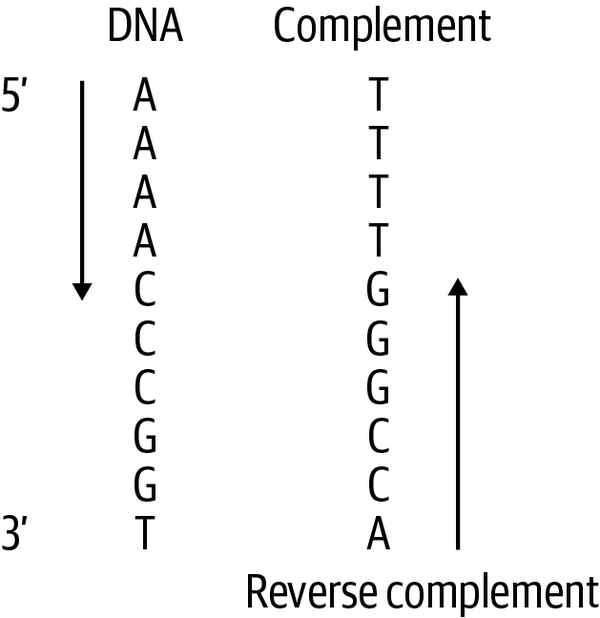
\includegraphics{images/reverse_complement.png}

This figure shows the reverse complement of a DNA sequence\footnote{\citet{clark2021}}

Training on DNA sequences and augmenting the data with their reverse complements has been shown to improve model accuracy, prediction, and interpretability in DNA sequence-related models. This approach involves ``treating the reverse complement DNA sequence as another sample'' \citep{cao2019}. By incorporating reverse complements, the model is exposed to a wider variety of sequence patterns, which helps reduce overfitting and enhances generalization. As a result, models become better at recognizing patterns regardless of strand orientation. Although the logic to obtain the reverse complement of a DNA strand is straightforward, the Bio.Seq module from the Biopython library provides a simple way to do this. Augmenting your dataset with reverse complements is usually done to training sets, but can be applied to validation and test sets as well.

\begin{Shaded}
\begin{Highlighting}[]
\ImportTok{from}\NormalTok{ Bio.Seq }\ImportTok{import}\NormalTok{ Seq}

\CommentTok{\# Example DNA sequence}
\NormalTok{dna\_sequence }\OperatorTok{=}\NormalTok{ Seq(}\StringTok{"ATGCGTAC"}\NormalTok{)}

\CommentTok{\# Generate the reverse complement}
\NormalTok{reverse\_complement }\OperatorTok{=}\NormalTok{ dna\_sequence.reverse\_complement()}

\BuiltInTok{print}\NormalTok{(}\StringTok{"Original Sequence: "}\NormalTok{, dna\_sequence)}
\end{Highlighting}
\end{Shaded}

\begin{verbatim}
## Original Sequence:  ATGCGTAC
\end{verbatim}

\begin{Shaded}
\begin{Highlighting}[]
\BuiltInTok{print}\NormalTok{(}\StringTok{"Reverse Complement: "}\NormalTok{, reverse\_complement)}
\end{Highlighting}
\end{Shaded}

\begin{verbatim}
## Reverse Complement:  GTACGCAT
\end{verbatim}

\textbf{Sequence Shifts}

Training on small, random sequence shifts up and downstream by shifting the genomic coordinates of the input sequence is also known as jitter. Jittering adds diversity to the training data by creating slightly different versions of the same sequence. This allows models to be less sensitive to the exact positioning of features, making them more robust to variations in the data. It also allows models to generalise better to unseen data where sites may not always be perfectly aligned. A variation of jittering, called flanking ``extends DNA sequences from its midpoint by X base pairs and takes the left, middle and right input windows of the extended sequence as training samples with the same labels, tripling the size of training set.\footnote{\citet{cao2019}}

Implementing data augmentations using reverse complements and sequence shifts can be approached in different ways. Similar to the `flanking' example, you can either expand your dataset by adding additional augmented data points or apply a random augmentation strategy, where only some data points are randomly augmented while keeping the total number of points in your dataset unchanged. Data augmentations are usually applied only to training sets, however in the context of computer vision ``many research reports have shown the effectiveness of augmenting data at test-time as well''.\footnote{\citet{connor2019}} When implementing augmentations like reverse complements and sequence shifts, these are typically applied after splitting your data into training, validation, and test sets. When applying sequence shifting, it's logical to shift the interval before retrieving the nucleotide sequence from the reference genome. The reverse complement should be applied after retrieving the nucleotide sequence but before one-hot encoding it. If you're using the BioPython library, this works well since BioPython's reverse complement function operates on string inputs.

In the genomics context, a paper on evaluating deep learning for predicting epigenomic profiles used two convolutional neural networks, \href{https://github.com/calico/basenji}{Basenji} and \href{https://github.com/kundajelab/bpnet}{BPNet}, trained on ATAC-seq data, to predict coverage values as a regression. They found that convolutional models trained with augmentations (reverse complement and sequence shifts), ``yielded improved robustness, especially when trained on peak-centered data (BPNet). On the other hand, models that were trained on coverage-threshold data (Basenji) already benefited from the randomly-centered profiles.''\footnote{\citet{toneyan2022}} Additionally, while they initially ``used a MSE and multinomial NLL loss for BPNet, {[}they{]} found that optimization using Poisson NLL yielded better performance.''\footnote{\citet{toneyan2022}} This finding is another motivation of using at poisson loss function in subsequent tutorials.

\section{Hyper-parameter optimisation}\label{hyper-parameter-optimisation}

Which learning rates are commonly used? How many epochs are typically used to train on?

While the learning rate and number of epochs differ by model and study, based on some of the research cited so far, common learning rates are in the range 1e-4\footnote{\citep{cedric2019}, \citep{avsec2021}} to 1e-3\footnote{\citep{cao2019}, \citep{toneyan2022}}. Additionally, some studies apply learning rate decay if the loss function shows no improvement over time\footnote{\citet{toneyan2022}} while others lower the learning rate for fine tuning.\footnote{\citet{avsec2021}}

The number of epochs used to train on differs by quite a margin. In training a convolution neural network to explore the effects of genomic data augmentation, 30 epochs were used.\footnote{\citet{cao2019}} DeepImpute which constructs multiple sub-neural networks for genotype imputation, trains on a maximum of 500 epochs, while the study involving the Basenji and BPNet models were trained on a maximum of 100 epochs. The clear strategy for these larger models involve the use of early stopping if no improvements are evident after 5-10 epochs.

When hyperparameter optimising, the consensus for achieving the best model performance is to train with a high number of epochs to enable the model to confidently learn features as they apply to labels, starting with a high learning rate, and decreasing over time using a learning rate scheduler. Interestingly, a study on binary peak detection using CNNs on ChIP-Seq data manually tuned their model's hyperparameters and found that little changes in performance results\footnote{\citet{oh2020}}. This highlights the challenges of hyperparameter tuning with larger models, where manually fine-tuning is not ideal. How can hyperparamter tuning on these larger models be done in practice?

\textbf{Raytune}

\href{https://docs.ray.io/en/latest/tune/index.html}{Raytune} ``is a Python library for experiment execution and hyperparameter tuning at any scale''. It aids in leveraging state of the art hyperparameter optmisation algorithms while simplifying scaling for larger models. Raytune hyperparameter searching can also be scaled to cloud based clusters without the need for large changes in code structure. Additionally, it supports several machine learning frameworks such as pyTorch and TensorFlow\footnote{\citet{liaw2018}}. One of the strongest current hyperparameter optmisation algorithms is the Asynchronous Successive Halving Algorithm or \textbf{\href{https://blog.ml.cmu.edu/2018/12/12/massively-parallel-hyperparameter-optimization/}{ASHA}}. Asha ``exploits parallelism and aggressive early-stopping to tackle large-scale hyperparameter optimization problems''\footnote{\citet{liam2018}}, allowing for faster optimisation and applicability to the larger models common in genomics. A study on predicting the impact of sequence motifs on gene regulation utilised Raytune and the ASHA algorithm to successfully optimise their model's hyperparameters\footnote{\citet{jacob2023}}.

In the genomic context, as a result of complex models using large genomic datasets, hyperparameter tuning using a brute force approach is untenable. Utilising existing libraries such as Raytune and incorporating asynchronous algorithms such as ASHA, has the potential to pave the way forward in improving model performance without unreasonable computational costs.

\chapter{Reproducibility of machine learning models}\label{reproducibility-of-machine-learning-models}

\section{Seeding}\label{seeding}

\section{Dashboarding}\label{dashboarding}

\chapter{Testing}\label{testing}

\chapter{Choosing which genomic regions to train on}\label{choosing-which-genomic-regions-to-train-on}

\chapter{Effect of differences in sequencing depths}\label{effect-of-differences-in-sequencing-depths}

\part{Software libraries for model building}\label{part-software-libraries-for-model-building}

\chapter{gReLU}\label{grelu}

\chapter{Kipoi}\label{kipoi}

\chapter{Weights and Biases}\label{weights-and-biases}

\part{ML pitfalls in genomics}\label{part-ml-pitfalls-in-genomics}

\chapter{Pitfalls overview}\label{pitfalls-overview}

\section{Distributional differences}\label{distributional-differences}

\section{Dependent examples}\label{dependent-examples}

\section{Confounding}\label{confounding}

\section{Leaky pre-processing}\label{leaky-pre-processing}

\section{Unbalanced classes}\label{unbalanced-classes}

In genomics, imbalance is a frequent challenge, often necessitating the use of statistical methods to validate the few positive instances amid vast amounts of data. In these cases, models can threaten to over-learn the majority class and under-learn the minority class. This is particularly evident in tasks such as alignment queries, GWAS projects, and motif scanning, where conservative significance thresholds are essential to control false positives due to the low frequency of true positives across the genome. The extensive size of the human genome exacerbates this issue, especially in problems related to non-coding variants, such as predicting chromatin states, gene expression, and disease status from sequence data.

Researchers address this imbalance by employing balancing algorithms that oversample the negative class and undersample the majority class. For instance, in training models to predict functional peaks from ChIP-seq or chromatin accessibility data, an approach might involve using all identified peaks along with a matching number of negative regions, thus effectively undersampling the majority class. For datasets with no such negative regions, researchers have to construct their own. While such imbalances are commonly discussed in classification, they also pose challenges in regression models predicting quantitative outcomes, where performance may be compromised in regions with sparse data, such as genomic areas or genes with low read counts in single-cell genomics studies.
\#\# Balancing the proportion of peaks / no-peaks in validation sets

\url{https://colab.research.google.com/drive/1wWlFffwBpOuK9yyCWp1hY6oiG9FK_6aX?usp=sharing}

\url{https://colab.research.google.com/drive/17xdEjl6TDew8Fb-bZvjRMIQSZX5s95Ae?usp=sharing}

\part{Model interpretability}\label{part-model-interpretability}

\chapter{Creating and visualising a simple model}\label{creating-and-visualising-a-simple-model}

\chapter{TF mo-Disco}\label{tf-mo-disco}

\part{Using existing models}\label{part-using-existing-models}

\chapter{Using the gReLU model zoo}\label{using-the-grelu-model-zoo}

\chapter{Fine tuning of Enformer}\label{fine-tuning-of-enformer}

\part{Predicting in novel cell types}\label{part-predicting-in-novel-cell-types}

\chapter{Incorporating ATAC-seq info}\label{incorporating-atac-seq-info}

\chapter{Use of cell type averages}\label{use-of-cell-type-averages}

\part{More complex models}\label{part-more-complex-models}

\chapter{Training multi-headed models}\label{training-multi-headed-models}

\chapter{Training siamese twin models}\label{training-siamese-twin-models}

  \bibliography{book.bib,packages.bib}

\end{document}
